\documentclass[10pt]{article}

\usepackage[left=1in,right=1in,top=1in,bottom=1in]{geometry}
\usepackage{amssymb}
\usepackage{enumitem}
\usepackage{graphicx}
\usepackage{array}
\usepackage[utf8]{inputenc}
\usepackage{enumitem} % Gives [resume]
\usepackage{mathtools}
\usepackage{empheq}
\usepackage{tikz}
\usepackage{hyperref}
\usetikzlibrary{automata,positioning,arrows.meta,calc}
\hypersetup{
    colorlinks=true,
    linkcolor=blue,
    filecolor=magenta,      
    urlcolor=cyan,
}
 
\urlstyle{same}

% Format for answering questions
\newenvironment{answer}
    {\begin{center}
    \begin{tabular}{|p{0.9\textwidth}|}
    \hline
    }
    { 
    \\\hline
    \end{tabular} 
    \end{center}
    }
 

\begin{document}

\title{CS 4341: Homework 3}
\author{Adam Camilli (aocamilli@wpi.edu)}
\date{\today}
\maketitle



\section*{Decision Tree:}
\begin{enumerate}
\item \textbf{Problem 18.6:} Consider the following data set comprised of three binary input attributes $(A_1,A_2,A_3)$ and one binary output:
  \begin{center}
  \begin{figure}[h!]
    \centering
    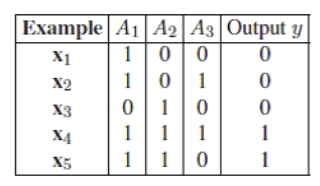
\includegraphics[width=0.7\textwidth,height=3cm,keepaspectratio]{hw3_3.png}
  \end{figure}
\end{center}
  Use the algorithm in Figure 18.5 (p. 702) to learn a decision tree for these data. Show the computations made to determine the attribute to split at each node.
  \begin{center}
  \begin{figure}[h!]
    \centering
    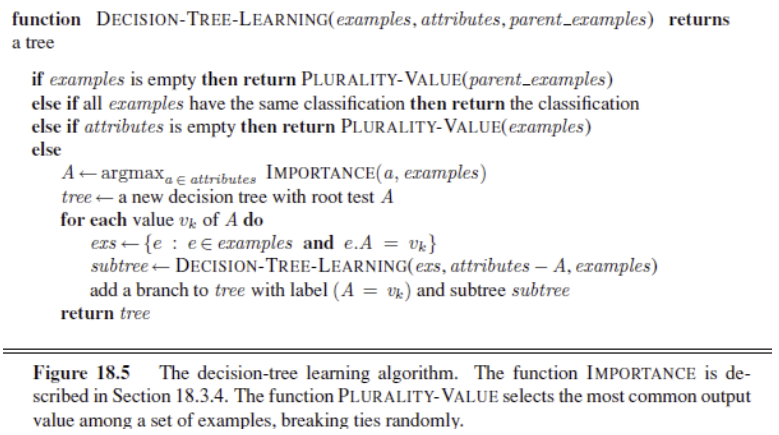
\includegraphics[width=0.9\textwidth,height=6cm,keepaspectratio]{hw3_4.png}
  \end{figure}
\end{center}
\begin{answer}
  Calculate the value of the remainder for each attribute in the first split, since provided info is before that.
  \[ A_1 = \frac{4}{5}\cdot \left(\frac{-2}{4}\log_2\left(\frac{2}{4}\right)\right) + \frac{1}{5}\left(-0-\frac{1}{1}\log_2\left(\frac{1}{1}\right)\right) = 0.8 \]
  \[ A_2 = \frac{3}{5}\cdot \left(\frac{-2}{3}\log_2\left(\frac{2}{3}\right)\right) + \frac{2}{5}\left(-0-\frac{2}{2}\log_2\left(\frac{2}{2}\right)\right) \approx 0.551 \]
  \[ A_3 = \frac{2}{5}\cdot \left(\frac{-1}{2}\log_2\left(\frac{1}{2}\right)\right) + \frac{3}{5}\left(\frac{-1}{3}\log_2\left(\frac{1}{3}\right)-\frac{2}{3}\log_2\left(\frac{2}{3}\right)\right) \approx 0.951 \]
Since $A_2$ is the minimum after the first split, the values for $A_2 = 0$ are classified as zero and so $X_1,X_2$ are ignored. The remaining $X_3,X_4,X_5$ are considered, all of which have $A_2=1$. Perform split on $A_2$, and then calculate remainders for $A_1,A_3$:
\[ A_1 = \frac{2}{3}\cdot \left(\frac{-1}{1}\log_2\left(\frac{1}{1}\right) - 0 \right) + \frac{1}{3}\left(-0-\frac{1}{1}\log_2\left(\frac{1}{1}\right)\right) = 0 \]
\[ A_3 = \frac{1}{3}\cdot \left(\frac{-1}{1}\log_2\left(\frac{1}{1}\right) - 0 \right) + \frac{2}{3}\left(\frac{-1}{2}\log_2\left(\frac{1}{2}\right) - \frac{1}{2}\log_2\left(\frac{1}{2}\right)\right) \approx 0.667 \]
Therefore we select $A_1$ for the split because all remaining examples are correct.
\end{answer}

\item Consider the following \textit{Play Tennis} dataset (adapted from: Quinlan, ``Induction of Decision Trees'', Machine Learning, 1986): \\
  \begin{center}
    \begin{minipage}[c]{0.4\linewidth}
      ATTRIBUTES: \\
      Outlook \\
      Temperature \\
      Humidity \\
      Wind \\
      PlayTennis \\
    \end{minipage}
    \begin{minipage}[c]{0.4\linewidth}
      POSSIBLE VALUES: \\
      \{Sunny, Rain, Overcast\} \\
      \{Hot, Mild, Cool\} \\
      \{High, Normal\} \\
      \{Strong, Weak\} \\
      \{Yes, No\} \hspace{1cm} $\leftarrow$ classification target \\
    \end{minipage}
    \newline
    \begin{tabular}{|c|c|c|c|c|c|}
      \hline
      ID & \textbf{Outlook} & \textbf{Temperature} & \textbf{Humidity} & \textbf{Wind} & \textbf{PlayTennis} \\
      \hline
      1 & Sunny & Hot & High & Weak & No \\
      \hline
      2 & Sunny & Hot & High & Strong & No \\
      \hline
      3 & Sunny & Hot & Normal & Weak & Yes \\
      \hline
      4 & Sunny & Mild & Normal & Strong & Yes \\
      \hline
      5 & Sunny & Mild & Normal & Weak & No \\
      \hline
      6 & Rain & Mild & High & Strong & No \\
      \hline
      7 & Rain & Mild & Normal & Weak & Yes \\
      \hline
      8 & Rain & Cool & Normal & Weak & Yes \\
      \hline
      9 & Rain & Mild & Normal & Strong & Yes \\
      \hline
      10 & Rain & Cool & Normal & Strong & No \\
      \hline
      11 & Overcast & Hot & High & Weak & Yes \\
      \hline
      12 & Overcast & Cool & High & Strong & Yes \\
      \hline
      13 & Overcast & Mild & High & Strong & Yes \\
      \hline
      14 & Overcast & Hot & Notmal & Weak & Yes \\
      \hline
      
    \end{tabular}
  \end{center}
  The machine learning task is to predict whether to play tennis or not, based on the data
  about the weather. Answer the questions in the following page.
  \begin{enumerate}
  \item Which of the major machine learning categories (supervised,
    unsupervised, or reinforcement) does this problem fall under?
    Explain. 
    \begin{answer}
      Since this problem already has a well-defined model with a set of variables and a domain for each, a given set of states, and does not involve any sort of rewards or incentives, it is classified as a supervised learning problem.
    \end{answer}
    Suppose we are in the middle of inducing the decision tree. The current state of the decision tree
    is given below:
    \begin{figure}[h!]
      \centering
      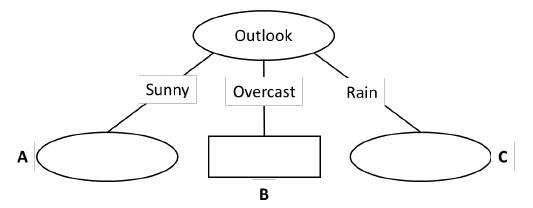
\includegraphics[width=\textwidth,height=5cm, keepaspectratio]{hw3_1.png}
    \end{figure}
    \item What should the tree output be in the leaf box labelled B? 
      \begin{answer}
        Since being Overcast does not preclude PlayingTennis, consider another attribute. The next one with the smallest domain are Humidity and Wind.
      \end{answer}
    \item Which data instances should be considered in node A? Write down the relevant instance
      ID numbers from the table.
      \begin{answer}
        Instances which are Overcast: 11,12,13,14
      \end{answer}
    \item Calculate the \textbf{entropy} at node A for the \textbf{Humidity} attribute. Show all the steps of your calculation. For your convenience, the logarithm in base 2 of selected values are provided.
      \begin{figure}[h!]
        \centering
        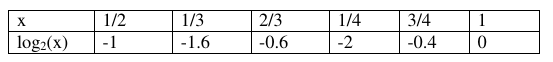
\includegraphics[width=0.7\textwidth,height=5cm,keepaspectratio]{hw3_2.png}
      \end{figure}
      \begin{answer}
        \[ \textrm{Entropy } = -\sum_iP_i\log_2P_i \]
        \[ \textrm{E(Sunny) + E(Sunny,High,Normal) } = -\frac{2}{5}(-1.32) - \frac{3}{5}(-0.74) + 0 + \frac{3}{3}(0) \approx 0.972 \]
      \end{answer}

    \item We have already calculated the entropies of Temperature and Wind at node A, and they
      are both 0.96. Based on these values, and based on the result you obtained previously,
      which attribute should be used to split node A? If needed, break any ties arbitrarily.
      \begin{answer}       
All three have equal probabilities (two values, split two and three) at node A. Since Humidity and Wind have the smallest domains, arbitrarily choose between them (i.e. Wind affects tennis more).
      \end{answer}
    \item Write your chosen attribute in the blank space of node A in the tree given in the previous
      page. Now extend the appropriate number of branches from node A and label them
      properly. For each branch that leads to a leaf, draw the leaf in the tree on the previous page
      and mark it with the output that the leaf should produce. Show your work on the tree on
      the previous page.
      \begin{figure}[h!]
        \centering
        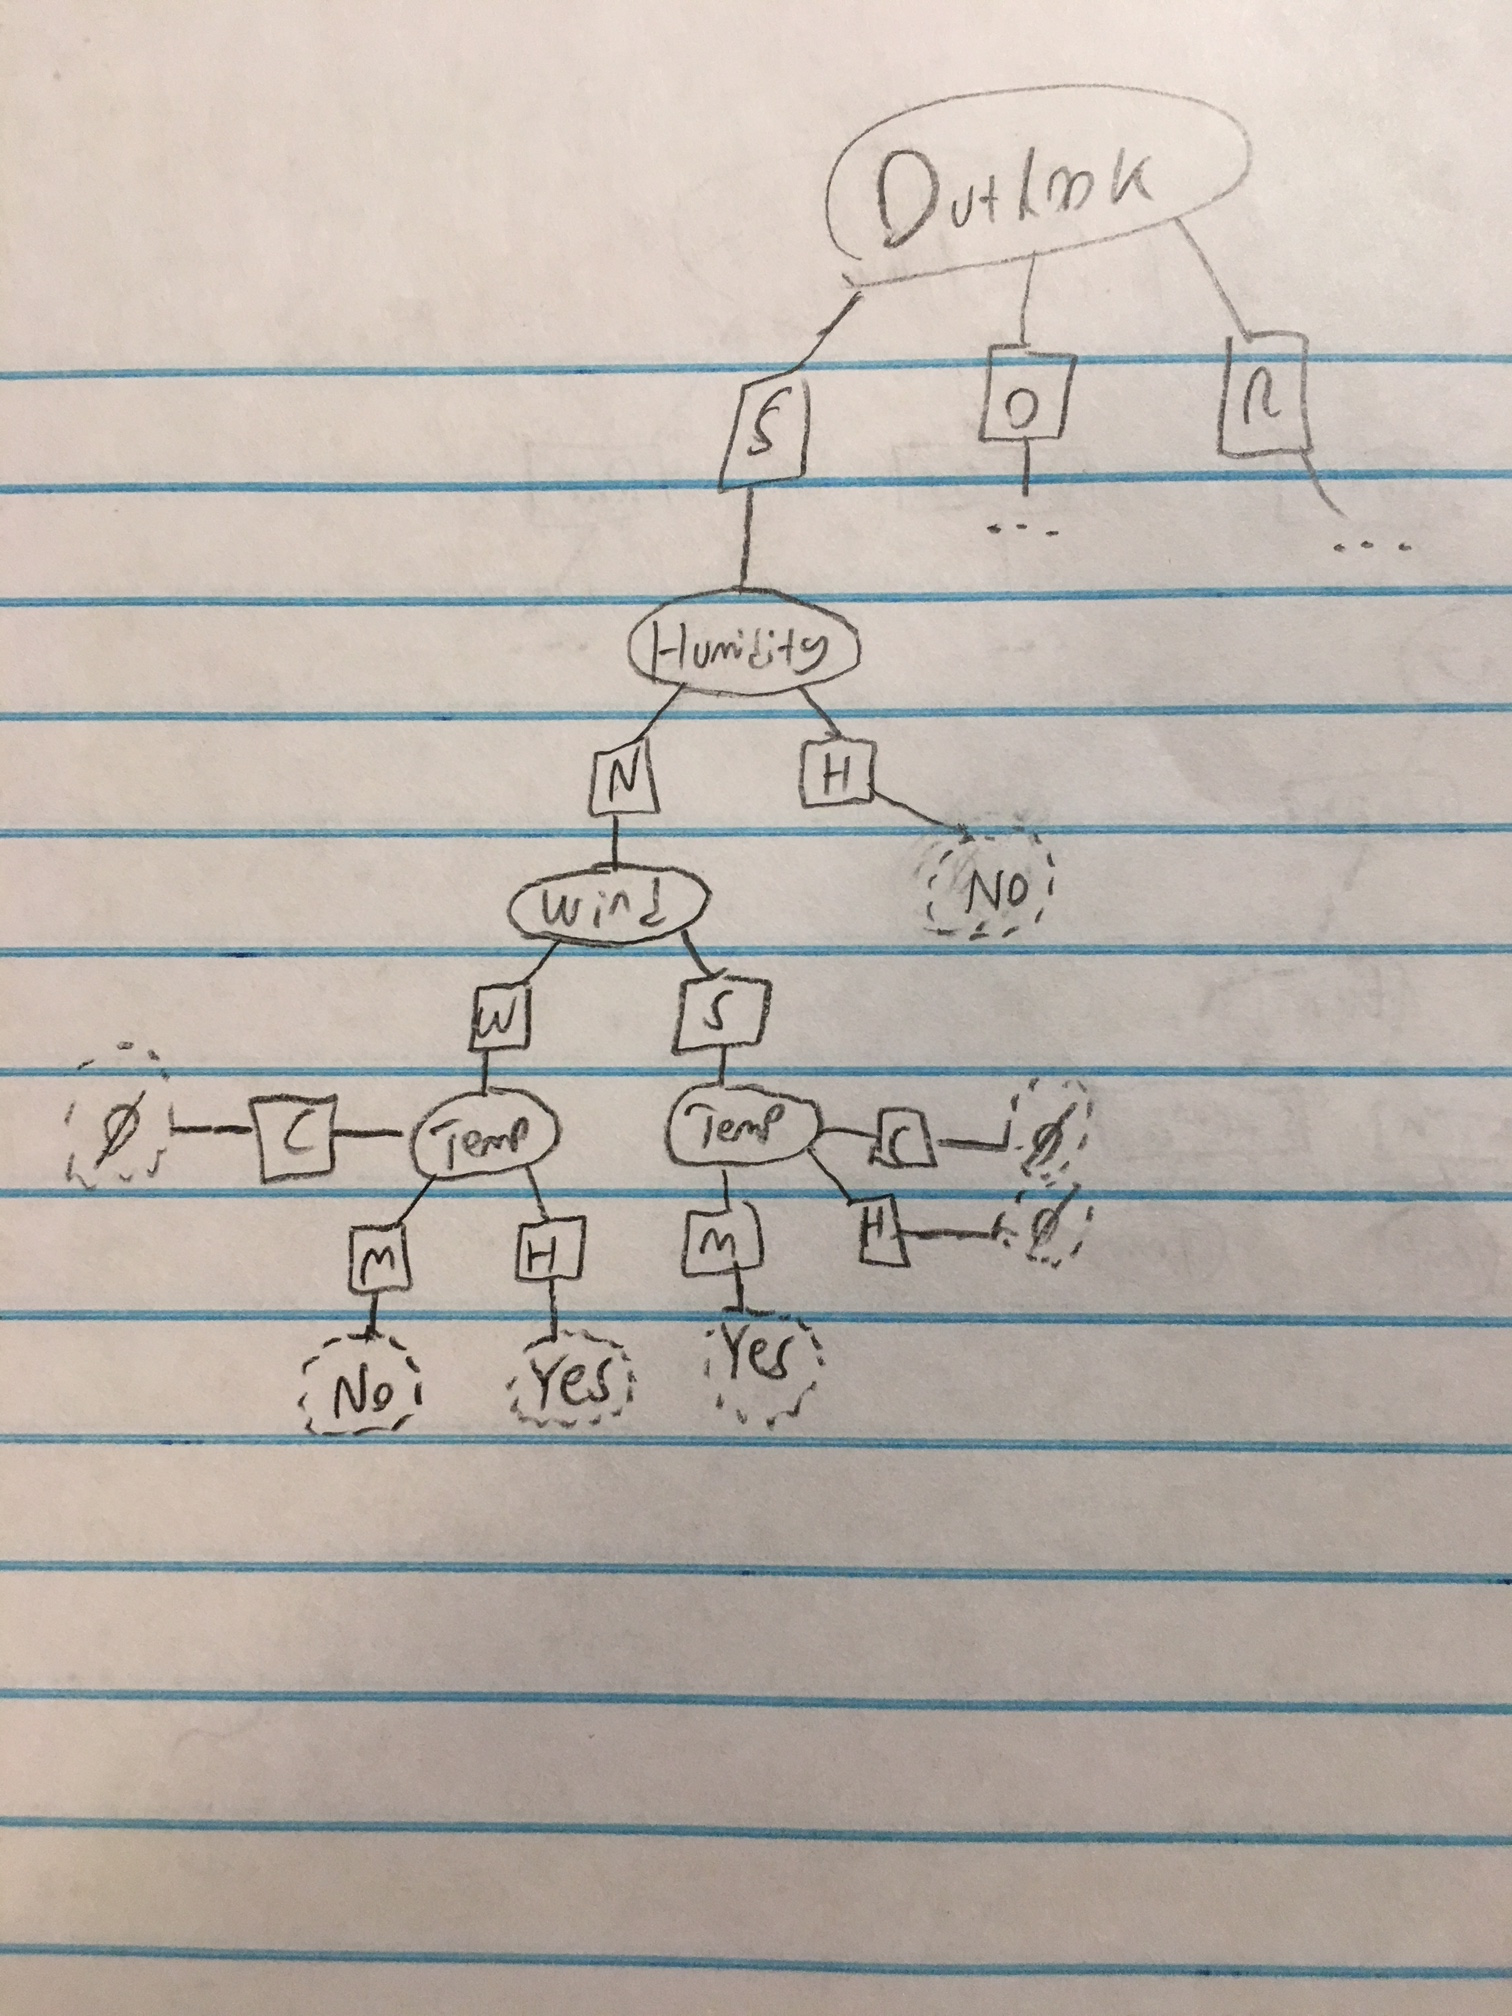
\includegraphics[width=0.7\textwidth,height=10cm]{hw3_13.jpg}
      \end{figure}
    \end{enumerate}  
  \end{enumerate}

  \section*{Naïve Bayes}
  \begin{enumerate}[resume]
  \item Use the \href{https://canvas.wpi.edu/files/1063366/download?download_frd=1}{Naive Bayes network in the class handout} to predict the Risk of the following data
    instance. Show your work.
    \begin{center}
      \textit{Credit History = bad; Debt = high; Collateral = adequate; and Income = >35.}
    \end{center}
    \begin{answer}
      \[ v = low: P(low)\cdot P(bad|low)\cdot P(high|low)\cdot P(adequate|low)\cdot P(>35|low) \]
      \[ v = \frac{3}{17}\cdot \frac{1}{8}\cdot \frac{3}{7}\cdot \frac{3}{7}\cdot \frac{6}{8}\cdot = \frac{162}{53312} \approx 0.003034 \]
      \[ v = mod: P(mod)\cdot P(bad|mod)\cdot P(high|mod)\cdot P(adequate|mod)\cdot P(>35|mod) \]
      \[ v = \frac{5}{17}\cdot \frac{3}{7}\cdot \frac{2}{6}\cdot \frac{2}{6}\cdot \frac{2}{7}\cdot = \frac{120}{29988} \approx 0.004002 \]
      \[ v = high: P(high)\cdot P(bad|high)\cdot P(high|high)\cdot P(adequate|high)\cdot P(>35|high) \]
      \[ v = \frac{6}{17}\cdot \frac{3}{8}\cdot \frac{5}{7}\cdot \frac{1}{7}\cdot \frac{1}{8}\cdot = \frac{90}{53312} \approx 0.001689\]
   Hence, the predicted value is Risk=moderate
    \end{answer}  
  \item Consider the same PlayTennis dataset of Problem 2, which is reproduced here for your
    convenience (though the data instances appear in a different order):
    \begin{figure}[h!]
      \centering
      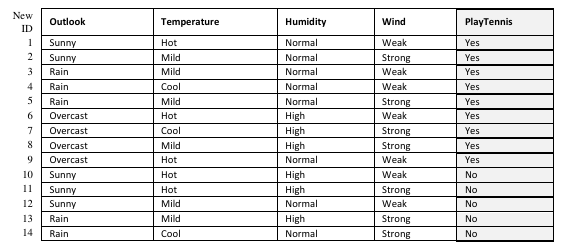
\includegraphics[width=0.8\textwidth,height=6cm]{hw3_5.png}
    \end{figure}
    \begin{enumerate}
    \item From the dataset above, the following Naïve Bayes model is built. Your job is to fill out the
      likelihood tables given below. Some tables have already been filled for your convenience.
      Remember that 1 is added to all the counts to avoid the problem of having a probability that is
      equal to 0 (Laplace smoothing).
      \begin{figure}[h!]
      \centering
      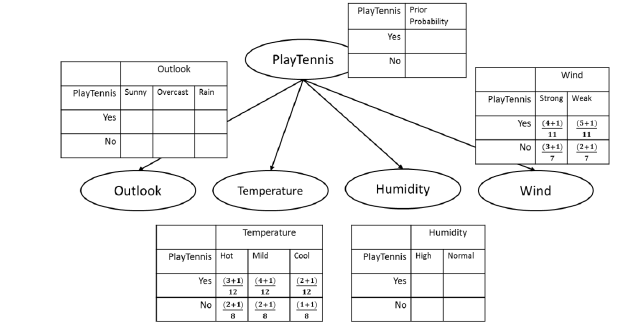
\includegraphics[width=0.9\textwidth,height=8cm]{hw3_6.png}
    \end{figure}
    \begin{answer}
      \\
      \begin{minipage}{0.6\linewidth}
        \begin{tabular}{|c|c|c|c|}
          \hline
          & \multicolumn{3}{|c|}{Outlook} \\
          \hline
          PlayTennis & Sunny & Outcast & Rain \\
          \hline
          Yes & $\frac{2+1}{5}$ & $\frac{4+1}{4}$ & $\frac{2+1}{5}$ \\
          \hline
          No & $\frac{3+1}{5}$ & $\frac{0+1}{4}$ & $\frac{3+1}{5}$ \\
          \hline
        \end{tabular}
      \end{minipage}      
      \begin{minipage}{0.1\linewidth}
        \begin{tabular}{|c|c|c|}
          \hline
          & \multicolumn{2}{|c|}{Humidity} \\
          \hline
          PlayTennis & High & Normal \\
          \hline
          Yes & $\frac{3+1}{6}$ & $\frac{6+1}{8}$ \\
          \hline
          No & $\frac{3+1}{6}$ & $\frac{2+1}{8}$ \\
          \hline
        \end{tabular}
      \end{minipage}
      \\
      \begin{center}
      \begin{minipage}{0.4\linewidth}
        \begin{tabular}{|c|c|}
          \hline
          PlayTennis & Prior Probability \\
          \hline
          Yes & $\frac{9+1}{15}$ \\
          \hline
          No & $\frac{6+1}{15}$ \\
          \hline
        \end{tabular}
      \end{minipage}
    \end{center}
      \\
    \end{answer}
    \item Use the Naïve Bayes model constructed in the previous page to classify the following new instance.
      That is, determine which of the two values of PlayTennis (Yes or No) has the highest probability
      given the outlook, temperature, humidity and wind values of the given instance. \textbf{Show all your work and explain your answer.}
    \begin{figure}[h!]
      \centering
      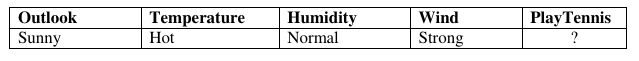
\includegraphics[width=0.7\textwidth,height=1cm]{hw3_7.png}
    \end{figure}
    \begin{answer}
      \[ v = No: P(No)\cdot P(Sunny|No)\cdot P(Hot|No)\cdot P(Normal|No)\cdot P(Strong|No) \]
      \[ v = \frac{7}{15}\cdot \frac{4}{5}\cdot \frac{3}{8}\cdot \frac{4}{6}\cdot \frac{4}{7}\cdot = \frac{1344}{25200} = \frac{4}{75} \approx 0.0533 \]
      \[ v = Yes: P(Yes)\cdot P(Sunny|Yes)\cdot P(Hot|Yes)\cdot P(Normal|Yes)\cdot P(Strong|Yes) \]
      \[ v = \frac{10}{15}\cdot \frac{3}{5}\cdot \frac{7}{8}\cdot \frac{4}{6}\cdot \frac{5}{7}\cdot = \frac{4200}{25200} = \frac{1}{6} \approx 0.1667 \]
      Yes has the highest probability.
    \end{answer}
    \end{enumerate}
  \end{enumerate}
  \section*{Artificial Neural Networks}
  \begin{enumerate}[resume]
  \item Investigate and explain the differences among the following types of "units" (i.e.,
    perceptrons) in terms of the activation functions that they use. In addition, provide a
    graphical depiction of these activation functions.
    \begin{itemize}
    \item Step
      \begin{answer}
        Most often used by the initial perceptron, useful for binary classification schemes or feature identifiers.
      \end{answer}
      \begin{figure}[h!]
        \centering
        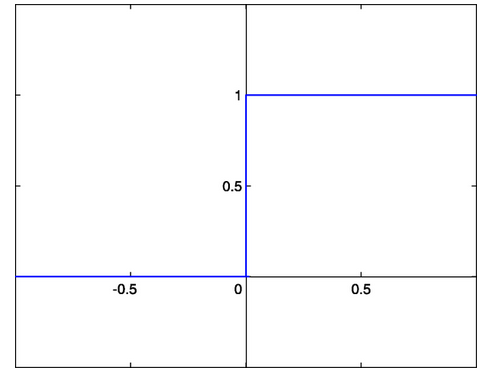
\includegraphics[width=0.4\textwidth,height=4cm]{hw3_8.png}
      \end{figure}
    \item Sigmoid
      \begin{answer}
        In order to stack layers and solve problems of non-trivial complexity, non-linearity must be introduced to a model. The sigmoid function is also used for classification schemes of real-world models that are not linear in nature. Since small changes in the parameters (X-values) propagate to huge changes in Y-values, the function usually brings activations to either side of the curve. Finally, the function is bound between (0,1), meaning no input will blow up the activations.
      \end{answer}
      \begin{figure}[h!]
        \centering
        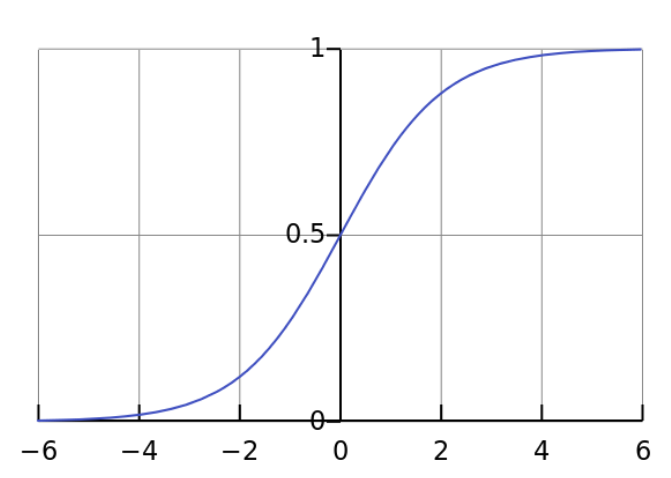
\includegraphics[width=0.4\textwidth,height=4cm]{hw3_9.png}
      \end{figure}
      \newpage
    \item ReLU
      \begin{answer}
        Again, ReLU is non linear, and so can be applied to real world scenarios. ReLU is used chiefly as an approximator, since combinations of it can approximate any function. It is not bound, and so activations can be blown up. Unlike sigmoid, however, the activations are sparse, and so most neurons in a network might not need to fire to get an output. This can be much more efficient with random initial inputs.
      \end{answer}
      \begin{figure}[h!]
        \centering
        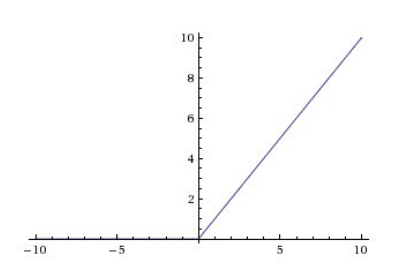
\includegraphics[width=0.6\textwidth,height=5cm]{hw3_10.png}
      \end{figure}
    \item Tanh
      \begin{answer}
        Tanh is essentially a scaled sigmoid function, used for the same purpose of classification. Due to its stronger gradient (steeper derivatives), tanh is even quicker to output towards 1 or 0.
      \end{answer}
      \begin{figure}[h!]
        \centering
        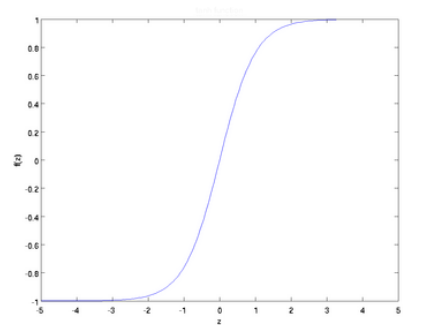
\includegraphics[width=0.4\textwidth,height=4cm]{hw3_11.png}
      \end{figure}
    \item Softmax
      \begin{answer}
        Softmax is often used in the final layer of a neural network classifier. It is used in multiple classification, since sigmoid cannot handle it. In addition to being bound between 0 and 1, the sum of all its outputs (probabilities) also approaches 1.
      \end{answer}
      \begin{figure}[h!]
        \centering
        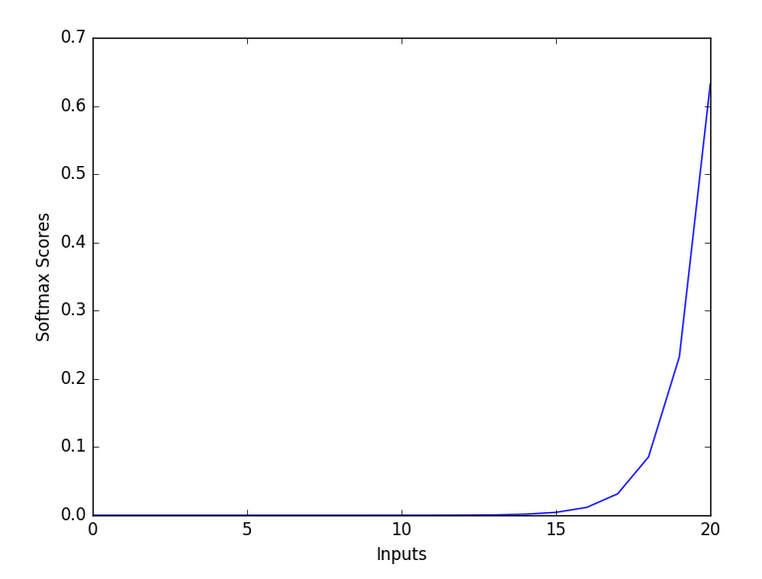
\includegraphics[width=0.4\textwidth,height=3cm]{hw3_12.png}
      \end{figure}
    \end{itemize}
    \newpage
  \item Problem \textbf{18.19} Construct by hand a neural network that computes the XOR function of two inputs. Be sure to specify what sort of units you are using.
    \begin{answer}
      Since XOR is essentially an OR with the AND case removed, it will be easiest to construct using steps of function units. An XOR function will have its network designed with OR, and the AND case will be computed with a hidden layer:
      \begin{center}
       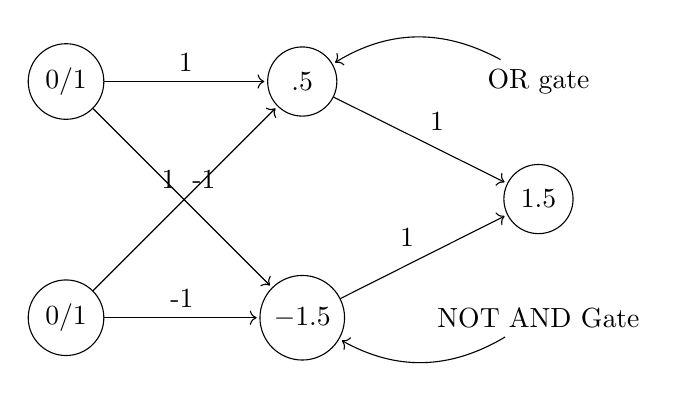
\begin{tikzpicture}[shorten >= 1pt, node distance = 3cm, auto]
         \node[state] (q0) {$0/1$};  %starting node
         \node[state] (q1) [right of=q0] {$.5$};
         \node[state] (q3) [below of=q0] {$0/1$};
         \node[state] (q2) [below of=q1] {$-1.5$}; 
         \node[state] (q4) [right of=q1, below=0.6cm of q1] {$1.5$};
         \node (orgate) [right of=q1] {OR gate};
         \node (andgate) [right of=q2] {NOT AND Gate};

         \path[->] 
         (q0) edge node {1} (q1)
         (q0) edge node [align=left] {-1} (q2)
         (q3) edge node {1} (q1)
         (orgate) edge [bend right] node {} (q1) 
         (q3) edge node [align=left] {-1} (q2)
         (q1) edge node {1} (q4)
         (q2) edge node {1} (q4)
         (andgate) edge [bend left] node {} (q2);
       \end{tikzpicture}
     \end{center}
    \end{answer}
  \item Problem \textbf{18.22 (a, c)} from textbook [Here h = No. of nodes in hidden layer]: Suppose you had a neural network with linear activation functions. That is, for each unit the output is some constant c times the weighted sum of the inputs.
    \begin{enumerate}
    \item Assume that the network has one hidden layer. For a given assignment to the weights \textbf{w}, write down equations for the value of the units in the output layer as a function of \textbf{w} and the input layer \textbf{x}, without any explicit mention of the output of the hidden layer. Show that there is a network with no hidden units that computes the same function.
      \begin{answer}
        A neural network with a linear activation function has an output unit that is essentially c times the input weighted sums. Therefore, if the activation function is $g(x) + d$, we are considering for each node only $c_i$ and $d_i$. \\
        If the network has a hidden layer \textbf{w} as weight, \textbf{x} as input layer without considering the output of the hidden layer. To show that there is a network without hidden units, we first suppose the output of the hidden layer is:
        \[ HL_j = g\bigg(\sum_{k}w_{k,j}I_k\bigg) = c\sum_{k}w_{k,j}I_k+d \]
        Therefore the final output is:
        \[ O = g\bigg(\sum_{j}w_{j,i}HL_{j}\bigg) = c\bigg(\sum_{j}w_{j,i}\big(\sum_{k}w_{k,j}I_k+d\big)\bigg) + d \]
        The same function can be computed as a two-layered network using a one layer perceptron with the weights 
        \[w_{k,j} = \sum_{j}w_{k,j}w_{j,i} \]
        with an activation function
        \[ g(x) = c^2x+d\big(1 + c\sum_{j}w_{j,i}\big) \]
      \end{answer}
      \item $\ldots$
      \item Suppose a network with one hidden layer and linear activation functions has n input and output nodes and h hidden nodes. What effect does the transformation in part(a) to a network with no hidden layers have on the total number of weights? Discuss in particular the case $h << n$.
        \begin{answer}
          This network with $n$ input and $h$ hidden nodes will have $2hn$ weights, whereas the reduced network has $n^2$ weights. When $h << n$, the original network will consist of fewer weights and so represent the input and output maps much more efficiently. Thus, a network is faster than a reduced one, which is one of the many disadvantages of using a linear activation function.
        \end{answer}
    \end{enumerate}
  \end{enumerate}
  
  \section*{Evaluating Machine Learning Models}
  \begin{enumerate}[resume]
  \item Assume that the following confusion matrix was obtained from using a machine learning
    model to predict the classification of 24 test instances, where the target attribute is Risk,
    with possible values low, moderate, and high:
    \begin{center}
      \begin{minipage}{0.4\textwidth}
        {\fontfamily{qcr}\selectfont
          \raggedright{
            a \space b \space c <-- classified as \\
            4 \space 0  \space 1 | a = low \\
            0 \space 1  \space 3 | b = moderate \\
            1 \space 2 12 | c = high \\
          }
        }
      \end{minipage}
    \end{center}
    For each of the following metrics used in project 3, provide a formula that defines the
    metric, and calculate its value based on the confusion matrix above. Show your work.
    
    \begin{itemize}
    \item The model's classification accuracy.
      \begin{answer}
        Examining the matrix, we can see there were $4 + 1 + 12=17$ true positives (TP), and since the model does not involve rejection there are $17$ true negatives (TN) as well. There are $1+3+1+2=7$ false positives (FP), and again since there are no rejections this is the number of false negatives as well (FN).
        $$ACC = \frac{TP+TN}{TP + TN + FP + FN} = \frac{17+17}{17+17+7+7} \approx 70.83\%$$
      \end{answer}
    \item The model's classification error (= 100\% - model's classification accuracy).
      \begin{answer}
        \[CError = 100\% - 70.83\% = 29.167\%\]
      \end{answer}
    \item The model's precision for class=low.
      \begin{answer}
        \[ PRE = \frac{TP}{TP+FP} = \frac{4}{4+1} = 80\% \]
      \end{answer}
    \item The model's recall for class=moderate.
      \begin{answer}
        \[ REC = \frac{TP}{TP+FN} = \frac{12}{12+3} = 80\% \]
      \end{answer}
    \end{itemize}
  \end{enumerate}
\end{document}